
\section{Introduction}

The Lossy Compression WG was formed in response to \jira{RFC-325} with its charter
being \citedsp{LDM-582}.  In \jira{RFC-325} it was recognized that user 
experience would likely be unacceptably impacted by the long latency required to 
access some LSST image data.  Central to this concern is that the current data model 
does not support storage and serving of processed visit images (PVIs), i.e. the 
detrended, calibrated individual exposures from the survey.  Instead, users needing
such images would either have to rely on retrieval from tape media or regeneration
of the PVIs on-the-fly.

Previous analysis has indicated that retaining all processed images on disk would 
be too costly and therefore not feasible, unless lossy compression is applied. 
The same analysis did indicated that storing all raw data on disk (with a loss-less 
compression) is feasible.  The Lossy Compression WG was asked to investigate whether 
some pipeline products might be saved after applying a lossy compression algorithm 
without significantly degrading their suitablity for a wide range of scientific 
investigations.  Central to this is the need that the compressed products be small 
enough that the cost to store and serve these images could be met within a reasonable 
budget.  The benefit from storing compressed products would only be realized if those 
products were indeed useful for many users as it would free resources that otherwise
would be engaged in regenerating or serving a tape archive.

The LSST has traditionally avoided lossy compression for any of its image data products 
(including the large co-added images as well as templates retained for each data release). 
Anecdotal experience from the Dark Energy Survey (DES; which uses FPACK; \citet{PSW2009}) 
and other surveys (e.g. HSC) indicates that lossy compression can be applied, without 
loss of scientific fidelity.  \citet{PWH2010} have argued that none of the scientific 
information is lost in an astronomical image even with fairly drastic quantization 
(at levels as high as 0.5$\sigma$).  The tests used by \citet{PWH2010} were relatively 
idealized, in this note we describe the results from a small test using precursor data 
from HSC to provide a sense of how lossy compression might be applied for LSST.



\section{Methodology}

This investigation is not meant to address the specific file format(s) that might be
used to store LSST data (e.g.; FITS vs. HDF5).  The tests that have been made were performed
using images stored using FITS, mainly because the changes necessary could be used within 
the current LSST pipeline testing infrastructure.  The specific images used were a set of
HSC data that formed a modest depth patch on which pipeline regression testing was already 
being routinely performed in the development of the LSST pipelines (the {\it ci\_hsc} test set).  
For this test set there were 33 images/CCDs, from 11 visit/exposures, at two bands (HSC-R, HSC-I).
Included among these images are a 4 images near the edge of the HSC focal-plane, where 
vignetting causes a portion of the detector unusable for science.  These regions are 
masked and present very different noise characteristics but are useful because they show some 
caveats that must be considered when applying compression.

A change has been injected into the pipeline that allows for a quantization to be applied
to the science (and weight) images that are traditionally stored as floats.  Formally,
the quantization factor, q, determines the number of samples/subdivisions of some set
number, in this case the standard-deviation of the image pixel values that do not contain a 
detected source.  For a FITS image this is expressed as a scale factor (BSCALE) and the image 
pixel values are converted to the nearest integer multiple of this factor.  We then use existing
loss-less compression algorithms to compress the integer representation of the image
to achieve a compressed image.  Our tests varied the factor q from 4 to 128 (stepping by 
factors of 2).

Metrics are then obtained to understand the impact and efficacy of compression.  Broadly, 
these fall into three categories:
\begin{enumerate}
\item {\bf Image Compression benchmarks:} to measure the changes at the pixel level.  These
include: percent increase in noise/RMS, median difference, and number of pixels that change
by more than the quantization level (to catch cases where the integer representation is not 
able to capture the full dynamic range of the original images).

\item {\bf Catalog/Measurement benchmarks:} to measure the change of aggregate quantities
of interest for scientists using the images for scientific measurements.  The current
benchmarks being measured are source position, flux, and shape along with their associated
uncertainties.

\item {\bf Compression algorithm benchmarks:} to measure the compression factor achieved, along with
algorithm execution times for compression and decompression.
\end{enumerate}
In addition a second round of image and catalog benchmarks can also be obtained to assess
the changes that might be expected when compressed products are combined to form stacked
images from which astronomical source measurements are also obtained.


\section{Results}

\subsection{Single Image Compression Benchmarks}

At the image level, independent measurements of the noise in the original science 
and weight images (I$_{0}$, W$_{0}$) and the quantized versions (I$_{\rm q}$, W$_{\rm q}$) are made.
The algorithms used are independent of those that performed the estimates used to set the quantization.
In most cases we consider only pixels with FLAG=0 or FLAG=32 (which indicates the presence of a source)
as heavily masked regions often have values (particularly in the weight image) that can exceed the 
range accessible in the quantized images.  Figure~\ref{pixel_dist} shows the distributions of pixels
values for the science and weight planes from two images typical of those in the test set.

\begin{figure}
\centering
  \begin{minipage}{.45\textwidth}
    \centering
    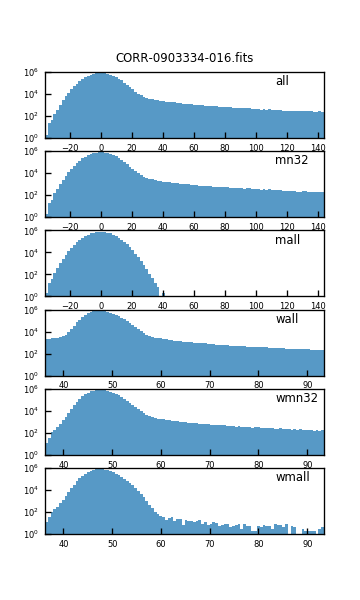
\includegraphics[width=1.0\textwidth]{figure/imgdist_CORR-0903334-016.fits.png}
%    \label{fig:sub1}
  \end{minipage}
  \begin{minipage}{.45\textwidth}
    \centering
    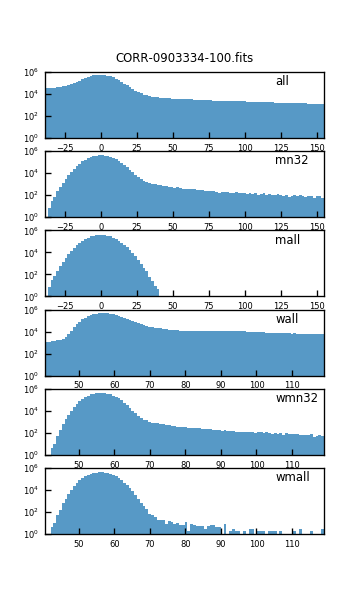
\includegraphics[width=1.0\textwidth]{figure/imgdist_CORR-0903334-100.fits.png}
%   \label{fig:sub2}
  \end{minipage}
\caption{Distributions of pixel values from two images in the test set. The left set of panels show 
distributions for a ``normal image'', while the right panels show the distributions for an image near the edge 
of the focal plane with heavy masking.  (top) to (bottom) the panels show: all science plane pixels (all), 
all science pixels with MASK=0 or 32 (mn23), and all unmasked pixels (mall), followed by similar
distributions for the weight plane (wall, wmn32, and wmall).  Note the "mall" and "wmall" are roughly
the distribution that was used to estimate the quantization level.}
\label{pixel_dist}
\end{figure}

A base level check is made that examines the difference between the quantized and unquantized version
of an image (${\rm I}_{\rm diff} = {\rm I}_{\rm q}-{\rm I}_{\rm 0}$).  First the mean, 
$\bar{\rm I}_{\rm diff}$, and RMS, $\sigma_{{\rm I}_{\rm diff}}$, are computed to show that no
systematic offset occurs and that the noise in the difference is indeed less than the scale factor.
We then also search for pixels where the difference exceeds the quantization level.  For most images
this latter value is identically zero but in a small number of cases the pixels in a bright object
will exceed the range available in the quantized image (i.e. the integer representation has insufficient
cardinality to track the dynamic range in the image).  If flagged pixels are included, then are typically
more pixels that exceed this range and in the worst cases (e.g. images from CCDs that are vignetted) a
large fraction of the weight pixels cannot be tracked.
{\bf More needed to quantitatively describe these?}

We then measure the standard deviation (RMS) in each science and weight image ($\sigma_{{\rm I}_{\rm q}}$ 
and $\sigma_{{\rm W}_{q}}$ respectively) to understand the fractional increase in the image noise
from the quantization ( $\sigma_{\rm grow} = \sqrt(\sigma_{{\rm I}_{q}}^2 - \sigma_{{\rm I}_{0}}^2 )$.  
Figures~\ref{image_difference} and \ref{weight_difference} show histograms of these metrics based
on the images in this test set.  The left panels show the residual noise as measured from the difference
between the unquantized and quantized images.  The right panels show the fractional additive noise 
resulting from the quantization.  Note that the number of samples in the histograms for q=64 and 128 
are smaller than the total because the measurement of the standard deviation is approaching the machine 
accuracy (i.e.  $\sigma_{{\rm I}_{q}}$ differs from $\sigma_{{\rm I}_{0}}$ by less than a part in 10$^{6}$).

\begin{figure}
\centering
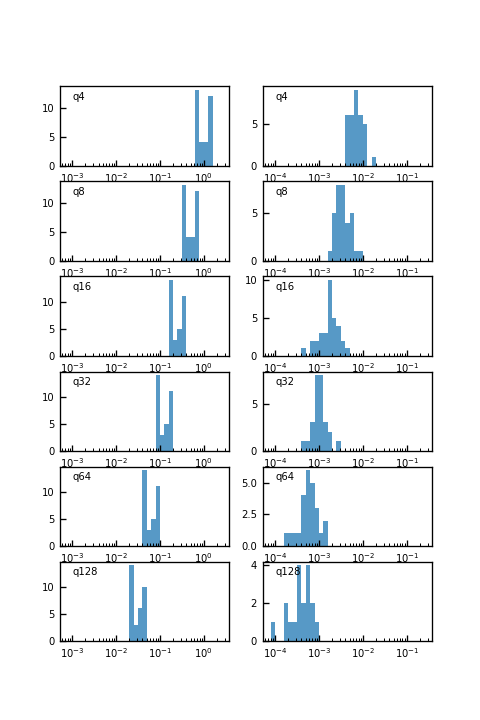
\includegraphics[width=0.75\textwidth]{figure/compression_metric_v2.png}
\caption{Histograms showing image level statistics with respect to the original compressed image.
(left panels) are histograms showing the RMS of the difference between the compressed and original image. 
(right panels) are histograms of the fractional increase in the noise with respect to the original image.}
\label{image_difference}
\end{figure}

\begin{figure}
\centering
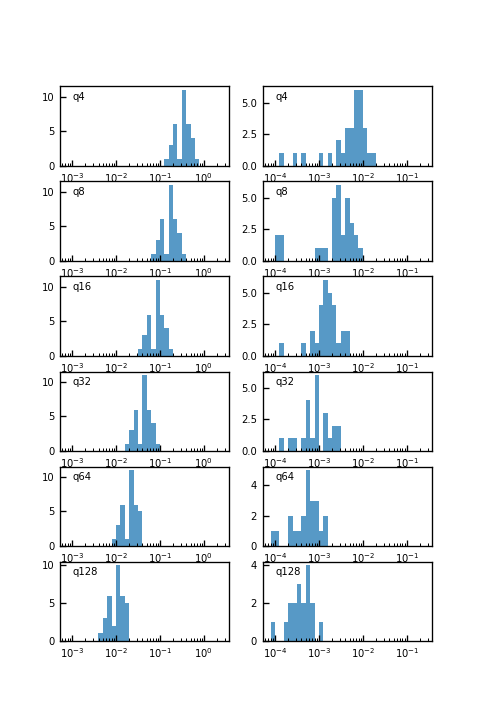
\includegraphics[width=0.75\textwidth]{figure/compression_metric_v2w.png}
\caption{Similar to Figure~\ref{image_difference} but for the weight image.}
\label{weight_difference}
\end{figure}


\subsection{Composite Image Benchmarks}

Beside the individual images, the current tests construct a coadded patch.  
Here, we compare the resulting coadd images constructured from the original, 
never-compressed images with coadd images constructed from the quantized images.
In the current limited test, only two coadded images (patches) were produced. 
The comparison is further hampered both because the depth of these coadd images 
is shallow (there are only 5 or 6 visits being combined per coadd) and an outlier 
rejection algorithm is active within the pipeline. This comparison is similar to 
that made for the individual images except that a a constraint has been added to 
remove locations where the clipping algorithm has systematically rejected a region 
of an image (in the test set there were of order a few such regions per coadd image
totalling comprised of a few times 10,000 pixels at q=4 dropping to ~1,000 pixels at q=64).

The results are summarized in Table~\ref{tab_agg_image_stat} which shows....
the 
% Currently this looks for 20-sigma outliers in the difference between quantized and unquantized (using clipped median and std-deviation) 

\begin{table}
\caption{Differences in Coadd Images Constructed from Quantized Images}
\centering
\begin{tabular}[]{crrrrrrrr}
\hline
 q        &  med($\delta_I$) & std($\delta_I$) & min($\delta_I$) & max($\delta_I$) & med($\delta_W$) & std($\delta_W$) & min($\delta_W$) & max($\delta_W$) \\
\hline
\multicolumn{9}{c}{Sample 1 (HSC-R coadd)}  \\
\hline
  q4    &  3.6$\times 10^{-5}$ & 1.3$\times 10^{-2}$ & -1.1$\times 10^{-1}$ & 9.0$\times 10^{-2}$ & $<10^{-6}$ & 3.8$\times 10^{-5}$ & -5.7$\times 10^{-4}$ & 5.7$\times 10^{-4}$ \\ 
  q8    & -4.0$\times 10^{-6}$ & 6.6$\times 10^{-3}$ & -5.3$\times 10^{-2}$ & 4.2$\times 10^{-2}$ & $<10^{-6}$ & 1.9$\times 10^{-5}$ & -2.8$\times 10^{-4}$ & 2.8$\times 10^{-4}$ \\
  q16   & -1.1$\times 10^{-5}$ & 3.3$\times 10^{-3}$ & -2.4$\times 10^{-2}$ & 2.1$\times 10^{-2}$ & $<10^{-6}$ & 1.0$\times 10^{-5}$ & -1.4$\times 10^{-4}$ & 1.4$\times 10^{-4}$ \\
  q32   &  3.0$\times 10^{-6}$ & 1.7$\times 10^{-3}$ & -1.4$\times 10^{-2}$ & 1.4$\times 10^{-2}$ & $<10^{-6}$ & 5.0$\times 10^{-6}$ & -7.1$\times 10^{-5}$ & 7.1$\times 10^{-5}$ \\
  q64   &  6.0$\times 10^{-6}$ & 8.3$\times 10^{-4}$ & -6.5$\times 10^{-3}$ & 5.6$\times 10^{-3}$ & $<10^{-6}$ & 2.0$\times 10^{-6}$ & -3.6$\times 10^{-5}$ & 3.6$\times 10^{-5}$ \\
  q128  &  2.0$\times 10^{-6}$ & 4.1$\times 10^{-4}$ & -3.4$\times 10^{-3}$ & 3.4$\times 10^{-3}$ & $<10^{-6}$ & 1.0$\times 10^{-6}$ & -1.8$\times 10^{-5}$ & 1.8$\times 10^{-5}$ \\
\hline 
\multicolumn{9}{c}{Sample 2 (HSC-I coadd)}  \\
\hline
  q4    &  4.4$\times 10^{-5}$ & 2.3$\times 10^{-2}$ & -1.7$\times 10^{-1}$ & 1.7$\times 10^{-1}$ & $<10^{-6}$ & 8.0$\times 10^{-5}$ & -1.1$\times 10^{-3}$ & 1.1$\times 10^{-3}$ \\
  q8    & -3.8$\times 10^{-4}$ & 1.2$\times 10^{-2}$ & -8.9$\times 10^{-2}$ & 8.4$\times 10^{-2}$ & $<10^{-6}$ & 4.0$\times 10^{-5}$ & -5.6$\times 10^{-4}$ & 5.6$\times 10^{-4}$ \\
  q16   & -3.4$\times 10^{-4}$ & 5.9$\times 10^{-3}$ & -4.3$\times 10^{-2}$ & 4.6$\times 10^{-2}$ & $<10^{-6}$ & 2.0$\times 10^{-5}$ & -2.8$\times 10^{-4}$ & 2.8$\times 10^{-4}$ \\
  q32   & -3.3$\times 10^{-4}$ & 3.1$\times 10^{-3}$ & -2.5$\times 10^{-2}$ & 2.5$\times 10^{-2}$ & $<10^{-6}$ & 1.0$\times 10^{-5}$ & -1.4$\times 10^{-4}$ & 1.4$\times 10^{-4}$ \\
  q64   & -3.3$\times 10^{-4}$ & 1.8$\times 10^{-3}$ & -1.8$\times 10^{-2}$ & 1.7$\times 10^{-2}$ & $<10^{-6}$ & 5.0$\times 10^{-6}$ & -7.0$\times 10^{-5}$ & 7.0$\times 10^{-5}$ \\
  q128  & -4.0$\times 10^{-6}$ & 7.3$\times 10^{-4}$ & -5.9$\times 10^{-3}$ & 5.2$\times 10^{-3}$ & $<10^{-6}$ & 2.0$\times 10^{-6}$ & -3.5$\times 10^{-5}$ & 3.5$\times 10^{-5}$ \\
\hline
\end{tabular}
\label{tab_agg_image_stat}
\end{table}





\subsection{Catalog/Measurement benchmarks}

Here we outline the comparison of measurements made on individual ccd-visit images with and without 
quantization applied.  Currently four types of measurements are considered: aperture photometry, 
PSF photometry, centroids, and shapes.  In each case the comparison is made by using forced 
photometry based on the COADD catalogs from the {\it ci\_hsc} run without quantization.
An astrometric match is made between the catalog from the never-quantized images to each of the
catalogs from the quantized images with a 1\arcsec\ match radius (with the nearest source being
considered the match).  The results from multiple CCDs are accumulated into a single plot in order
to obtain statistics at the bright end.

Figures~\ref{plot_se_flux} show comparisons for flux measurements for aperture photometry 
and PSF fitting.  The aperture photometry measurements {\it base\_CircularApertureFlux\_6\_0} 
use a 6 pixel radius circular aperture while the PSF fitting measurements are the
{\it base\_PsfFlux\_flux} measurements.  Note that in these plots no star-galaxy classifier 
was used to subselect stellar/point-source measurements.

The top two panels in each set show the total number of objects per flux bin, followed by a plot 
showing the flux uncertainty as a function of flux from the never compressed image.  Beneath these 
are plotted the difference between the measurements from the quantized images and the never-quantized 
images with subsequent plots using an increasing level of quantization.  These differnce 
plots are shown in units of $\sigma_{\rm F_0}$ (i.e. each difference measurement is scaled by the
uncertainty in the flux measured in the unquantized image).  Overplotted are histograms showing the 
diffence level that encompasses 50, 75, 90, and 99\% of the measurements as a function of flux bin.
{\bf Remove 99\% histogram?}
Careful examination of the histograms show that for quantization, q=16 or greater 50\% of all 
flux measurements differ by less than 0.01$\sigma$ and 90% by less than 0.1$\sigma$ when 
compared to the measurements on the unquantized images.

\begin{figure}[t]
\centering
    \begin{minipage}{.49\textwidth}
        \centering
        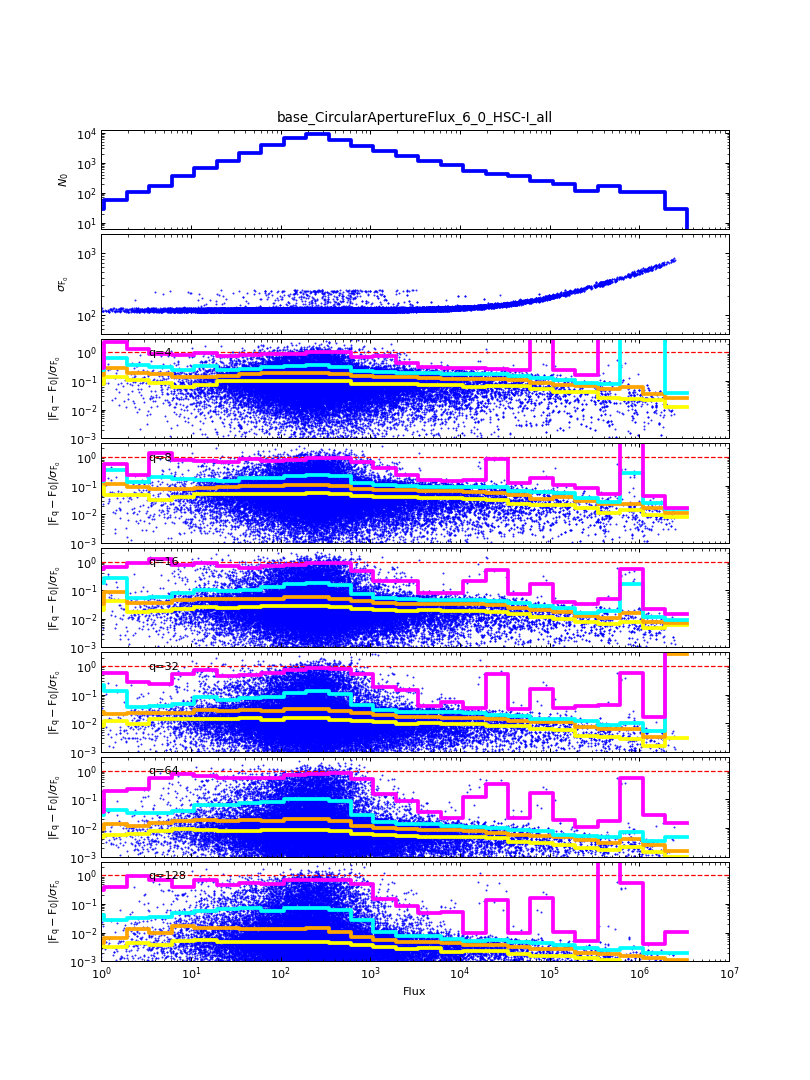
\includegraphics[width=1.0\textwidth]{figure/rplot_all_base_CircularApertureFlux_6_0_HSC-I.png}
%        \label{fig:sub1}
    \end{minipage}
    \begin{minipage}{.49\textwidth}
        \centering
        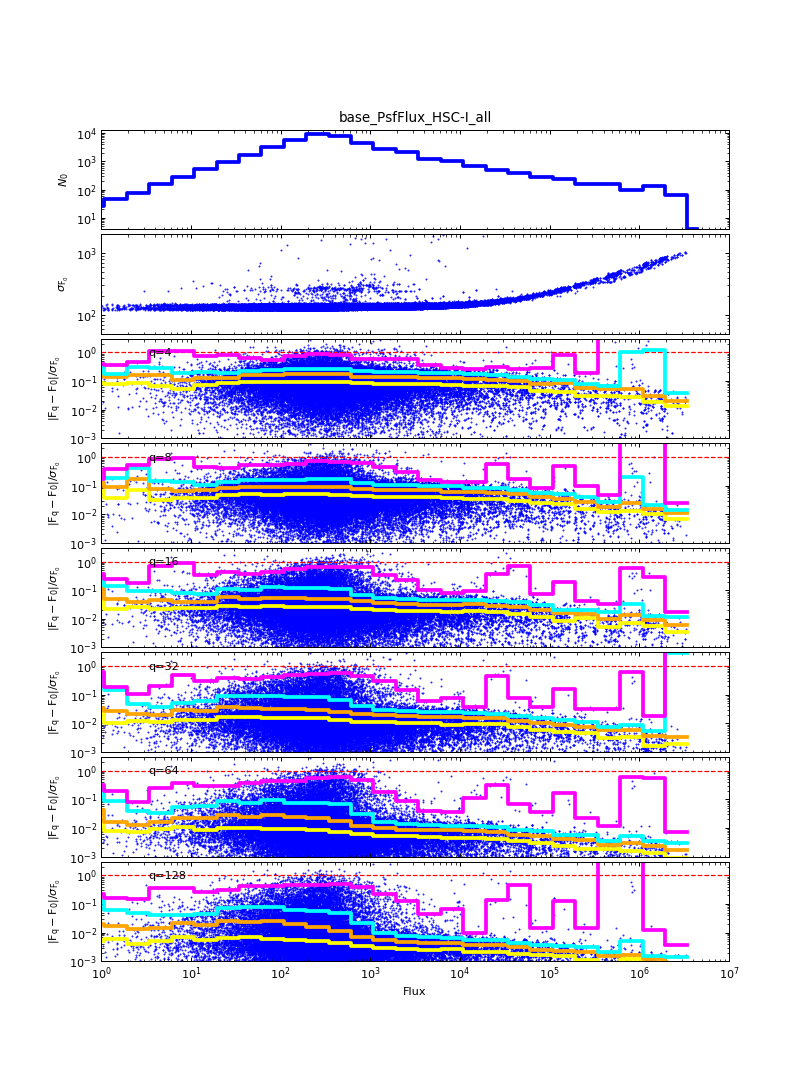
\includegraphics[width=1.0\textwidth]{figure/rplot_all_base_PsfFlux_HSC-I.png}
%        \label{fig:sub2}
    \end{minipage}
\caption{Comparison of aperture (left) and PSF photometry (right) measurements resulting from forced photometry 
on individual images with and without quantization/compression.  The top panel in each shows the distrubution 
of objects as a function of their flux measured in the original image(s).  The second plots show measure uncertainties 
for those flux measurements.  The panels below show the difference between the flux measurements made on the
unquantized and quantized images divided by the uncertainty in the quantized images (in units of $\sigma_{\rm F_0}$.  
A dashed horizontal red line shows the 1$\sigma$ difference level for reference.  The lower panels are for 
measurements from the images with progressively higher quantization factors (less loss).
The histograms in each panel show the difference level at which 50, 75, 90 and 90\% of the objects are found.}
\label{plot_se_flux}
\end{figure}


Similar to the flux measurements, Figure~\ref{plot_cen_shape} shows comparisons of centroid
and shape measuremnts (left and right panels, respectively) as a function of signal-to-noise
(S/N) in the unquantized images.  For the centroids we use the {\it base\_SdssCentroid\_x} (x), and 
{\it base\_SdssCentroid\_y} (y), to compute the linear offset 
$X_q-X_0 = \sqrt{ (x_q-x_0)^2 + (y_q-y_0)^2}$ between the measurments
made in the quantized and unquantized images.  Note that the current version of forced photometry 
does not flag poor and low signal-to-noise measurements so those measurements pollute/inflate the 
distributions show in the low signal-to-noise portion of the centroid plots in Figure~\ref{plot_cen_shape}.

In order to investigate the impact of quantization on shapes, we use the {\it base\_SdssShape\_xx}, 
{\it base\_SdssShape\_yy}, and {\it base\_SdssShape\_xy} measurements to form a shape measurement, 
$S$, where $S=(I_{xx} I_{yy} - I_{xy}^2)^{1/4}$.
Assuming that those 2nd moment measurements are not strongly correlated, we also define
the uncertainty in $S$ as 
$\sigma_S^2 = (\frac{\partial S}{\partial I_{xx}})^2 \sigma_{I_{xx}}^2 + 
(\frac{\partial S}{\partial I_{yy}})^2 \sigma_{I_{yy}}^2 + 
(\frac{\partial S}{\partial I_{xy}})^2 \sigma_{I_{xy}}^2$, and use the associated uncertainties
to estimate $\sigma_S$.  Figure~\ref{plot_cen_shape} shows these measurements and makes a comparison
of the quantized measurments to those found with the unquantized images.  Measurements with 
{\it base\_SdssShape\_flag} have been excluded.

Examination of the centroid plots in Figure~\ref{plot_cen_shape} show that for quantization of q=16 or
better the difference in centroid measurements is less than 0.1 pixels for 90\% of measurements for
sources with S/N$>$10.  Similarly, for shape measurements the differences in $S$ are already less than 
0.01 pixels for 90\% of objects at a S/N$>$10.  

\begin{figure}[t]
\centering
    \begin{minipage}{.49\textwidth}
        \centering
        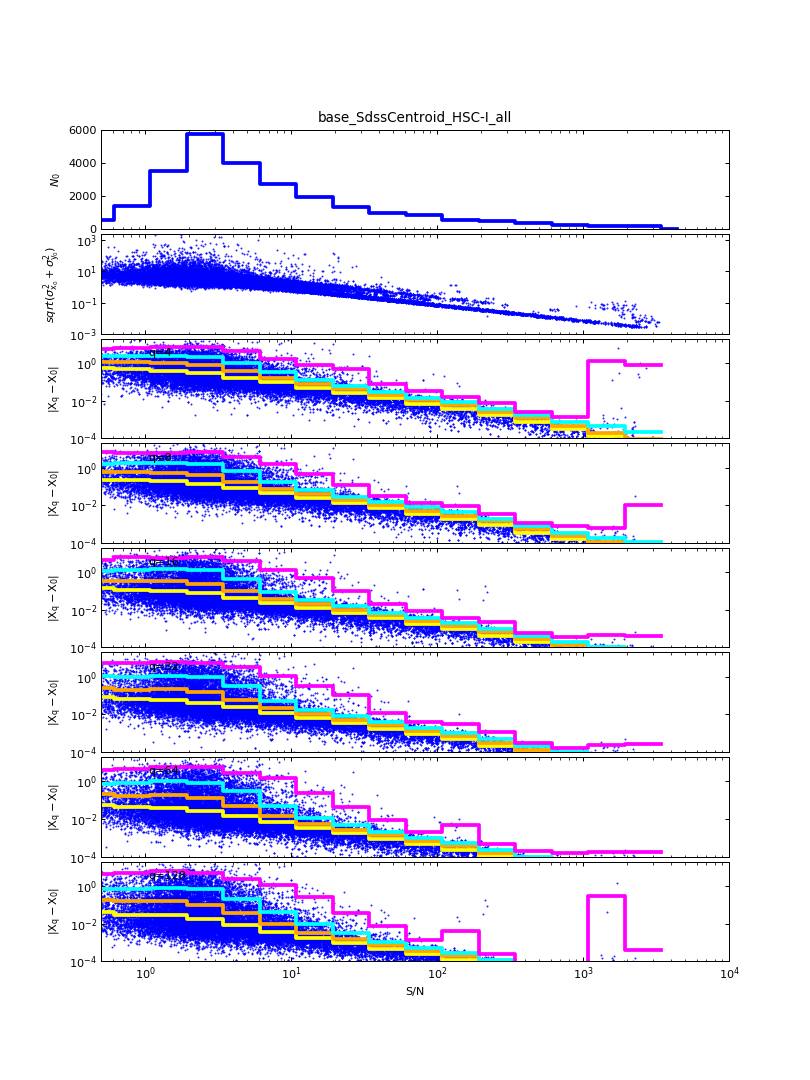
\includegraphics[width=1.0\textwidth]{figure/rplot_all_base_SdssCentroid_HSC-I.png}
%        \label{fig:sub1}
    \end{minipage}
    \begin{minipage}{.49\textwidth}
        \centering
        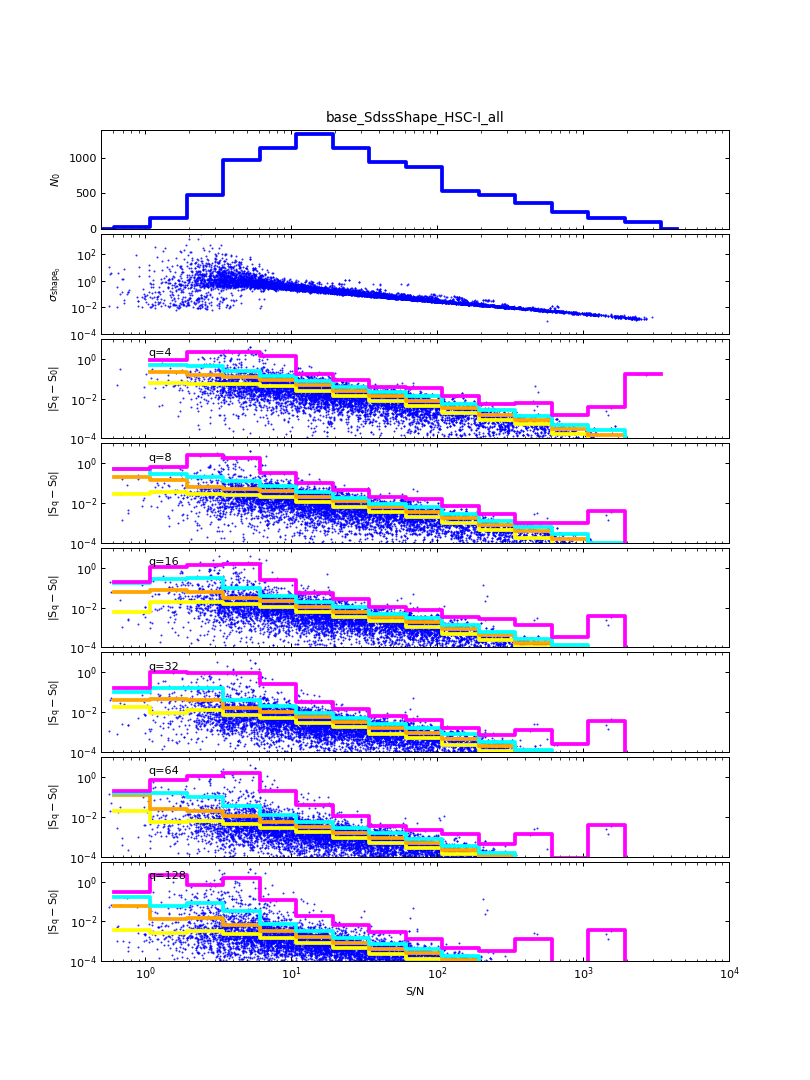
\includegraphics[width=1.0\textwidth]{figure/rplot_all_base_SdssShape_HSC-I.png}
%        \label{fig:sub2}
    \end{minipage}
\caption{Similar to Figures~\ref{plot_se_flux} but for centroid (left) and shape (right) measurements as function 
of the signal-to-noise ratio of the unquantized measurements.  The differences in the lower panels 
are in units of pixel offset and pixel radius for the centroid and shape measurements, respectively.}
\label{plot_cen_shape}
\end{figure}

%
%\begin{figure}
%\centering
%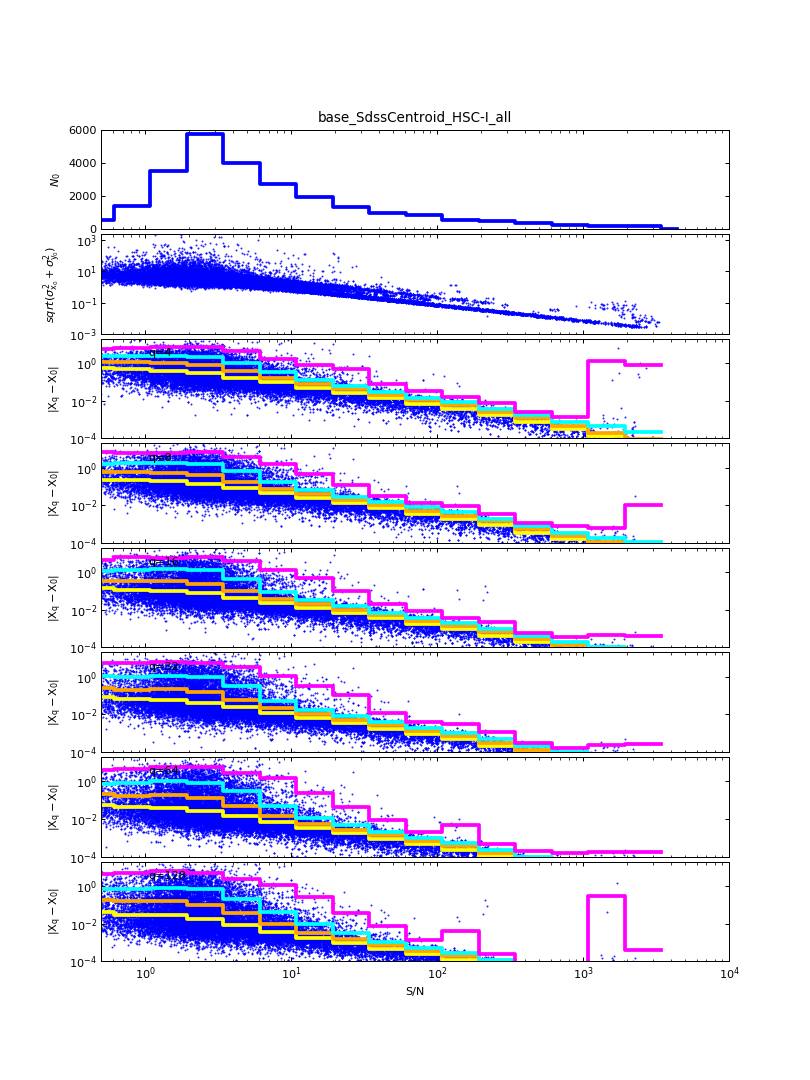
\includegraphics[width=0.75\textwidth]{figure/rplot_all_base_SdssCentroid_HSC-I.png}
%\caption{Similar to Figures~\ref{plot_app_flux}\&\ref{plot_psf_flux} but for centroid measurements as function of the signal-to-noise ratio
%of the unquantized measurements.  The differences in the lower panels are in units of pixel offset.}
%\label{plot_cen}
%\end{figure}
%
%\begin{figure}
%\centering
%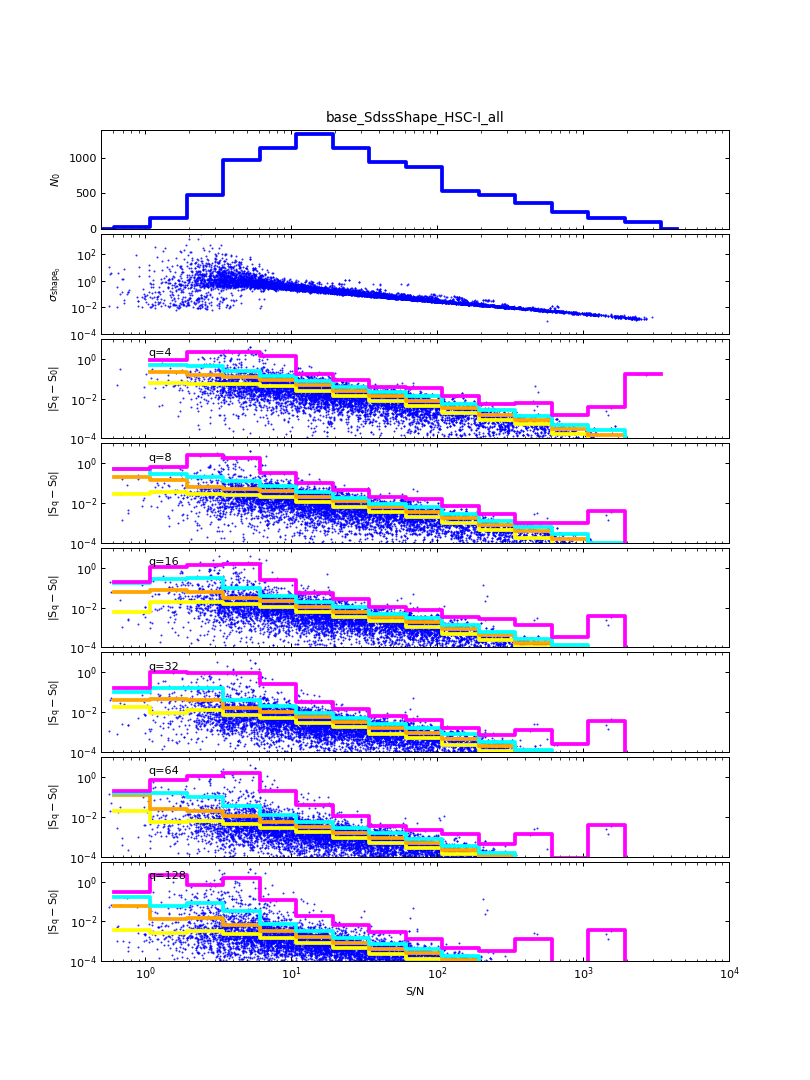
\includegraphics[width=0.75\textwidth]{figure/rplot_all_base_SdssShape_HSC-I.png}
%\caption{Similar to Figure~\ref{plot_cen} but for the SDSS shape measurments.  The comparison is made using the quantity S which is equivalent to
%a size/radius.}
%\label{plot_shape}
%\end{figure}




\subsection{Catalog/Measurement from COADD images constructed from quantized PVI images}

Similar to the comparisons made for the individual images, we compare the catalog measurements from the coadded patch
that was constructed from the never-quantized and the quantized PVI images.  Note, no further quantization/loss was applied
to the COADD images.  The same four quantities were examined (aperture flux, PSF flux, centroid, and shape).  
Figures~\ref{plot_coadd_flux} through \ref{plot_coadd_cen_shape} show the results of that comparison.


\begin{figure}[t]
\centering
    \begin{minipage}{.49\textwidth}
        \centering
        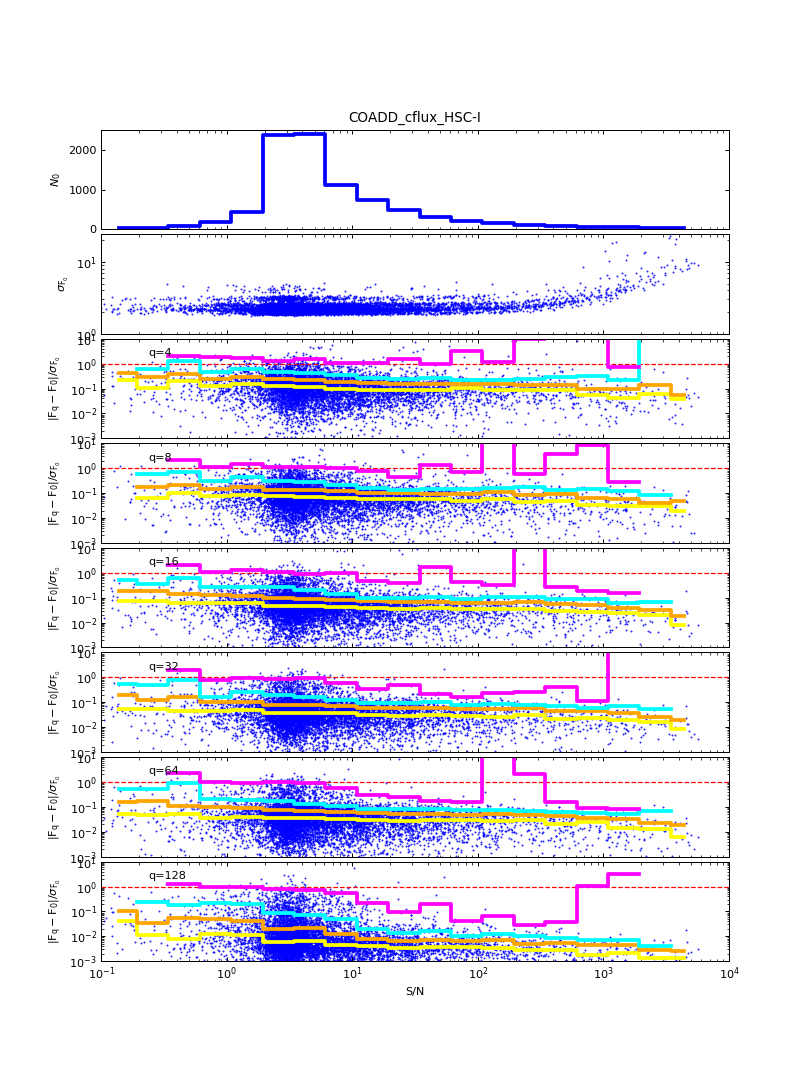
\includegraphics[width=1.0\textwidth]{figure/plot_coadd_cflux_HSC-I.png}
%        \label{fig:sub1}
    \end{minipage}
    \begin{minipage}{.49\textwidth}
        \centering
        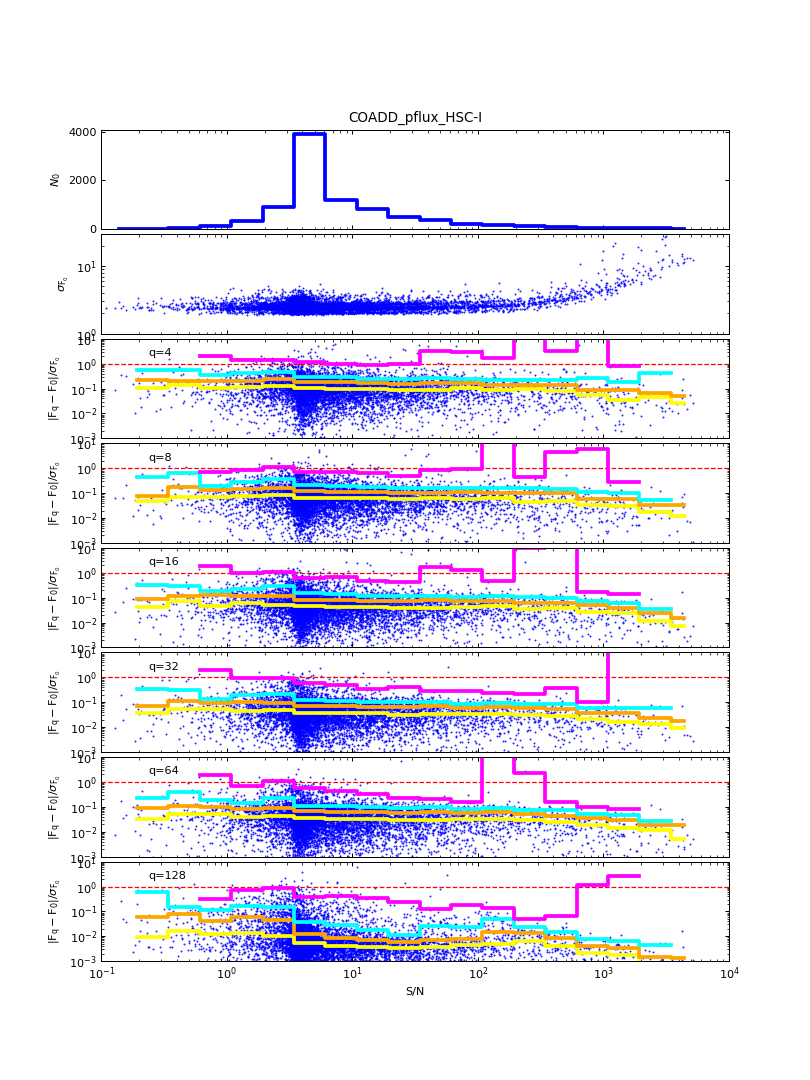
\includegraphics[width=1.0\textwidth]{figure/plot_coadd_pflux_HSC-I.png}
%        \label{fig:sub2}
    \end{minipage}
\caption{Similar to Figure~\ref{plot_se_flux} but for measurements made on the coadd image.}
\label{plot_coadd_flux}
\end{figure}


\begin{figure}[t]
\centering
    \begin{minipage}{.49\textwidth}
        \centering
        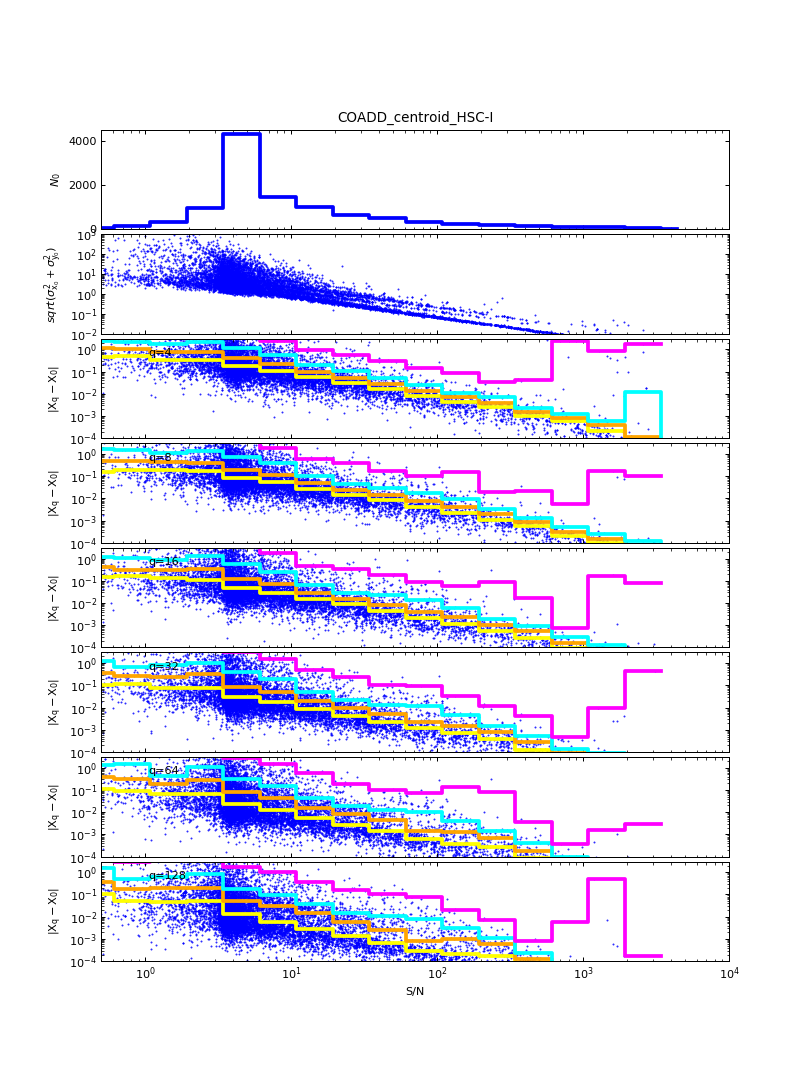
\includegraphics[width=1.0\textwidth]{figure/plot_coadd_centroid_HSC-I.png}
%        \label{fig:sub1}
    \end{minipage}
    \begin{minipage}{.49\textwidth}
        \centering
        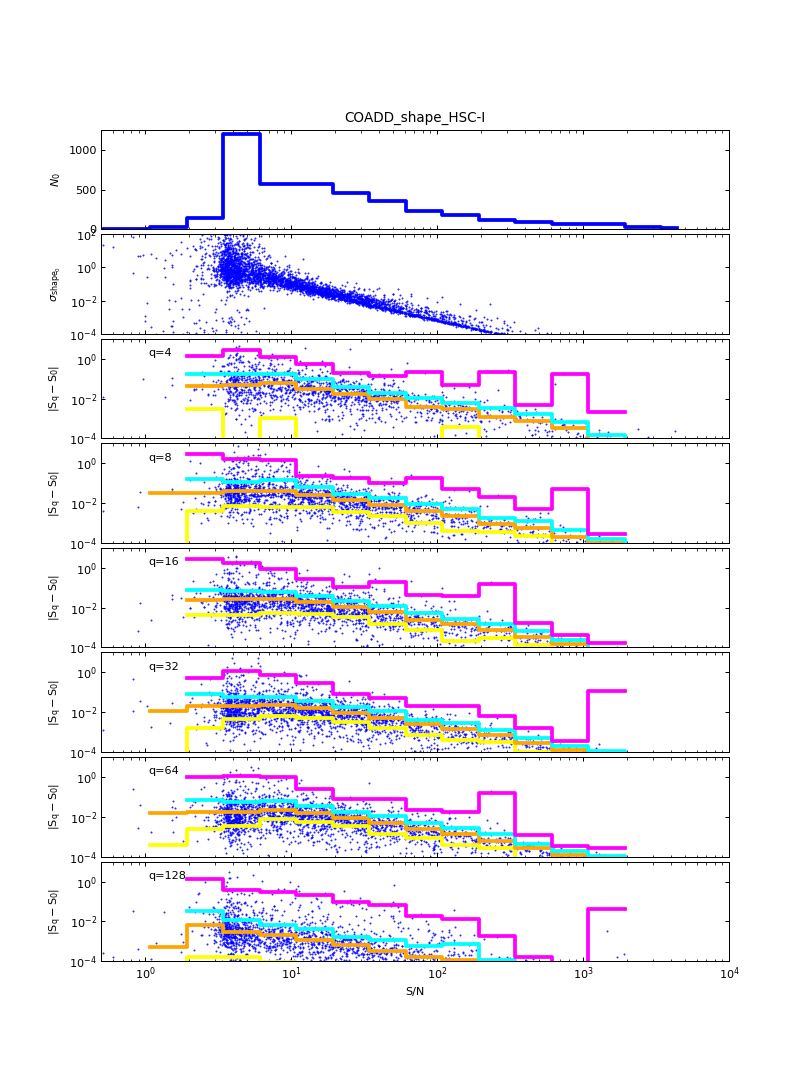
\includegraphics[width=1.0\textwidth]{figure/plot_coadd_shape_HSC-I.png}
%        \label{fig:sub2}
    \end{minipage}
\caption{Similar to Figure~\ref{plot_cen_shape} but for measurements made on the coadd image.}
\label{plot_coadd_cen_shape}
\end{figure}





\subsection{Compression Algorithm benchmarks}

We have applied a variety of existing compression algorithms to the quantized images from this study to 
obtain benchmarks of their efficacy.  The values reported reflect those algorithms' performance when
running under OS X 10.13.2 (macOS High Sierra) on a MacBook Pro with quad 2.9 GHz processors.  A ramdisk
was used for storage to minimize the impact of I/O operations within the test.  

A range of existing algorithms have been benchmarked, including a number which use threading to achieve 
greater speed.  The algorithms considered were:
\begin{enumerate}
\item {\bf gzip:} the standard GNU implementation of Lempel-Ziv (LZ77).
\item {\bf pigz:} a threaded version of gzip.
\item {\bf bzip2:} an implementation of Burrows-Wheeler block sorting (offers the possibility of recovery of undamage block).
\item {\bf pbzip2:} a threaded/parallel implementation of bzip2.
\item {\bf lbzip2:} another threaded/parallel implementation of bzip2.
\item {\bf lz4:} a "typically faster" implementation of LZ77 (favoring speed over compression ratio). Pushing to higher compression ratios significantly degrades performance.
\item {\bf lzop:} a separate implementation that trades a small hit in compression time for an improvement in decompression.  The performance trade is not apparent at the file size being used in these tests.
\item {\bf zstd:} Also based on the LZ77 family and includes a parallel implementation.  In addition this
algorithm has implementations/bindings over a wide variety of languages (including Python).  
The usage of a pre-computed dictionary may offer improvement in speed/compression factor but 
rigorous testing was not possible for this small set (performance was identical to the untrained
algorithm if the full set was used both to train and then obtain benchmarks).
\item {\bf xz:} 
\end{enumerate}

The results from benchmark tests are summarized in Tables~\ref{compress_factor}-\ref{timing_decompress}, 
showing compression factor, time to compress per file, and time to decompress per file, respectively.
These times do not include the time to necessary to obtain and apply scale factor used in the quantization.  Furthermore, the set of files being compressed are nearly identical (98 Mb) and therefore do not provide 
any information about algorithmic performance with respect to file size.  When a parallel implementation
was available the threading was set to use 4 cores.


\begin{table}
\caption{Compression Factor Achieved}
\centering
\begin{tabular}[]{crrrrrrrrr}
\hline
 q        &  gzip & pigz & bzip2 & pbzip2 & lbzip2 & lz4 & lzop & zstd & zstdb  \\
\hline
 q4       &   6.73 &  6.73 &  9.96 &  9.95 &  9.96 &  3.69 &  3.11 &  6.29 &  6.29  \\
 q8       &   5.54 &  5.53 &  8.20 &  8.20 &  8.21 &  3.34 &  2.96 &  5.42 &  5.42  \\
 q16      &   4.69 &  4.69 &  6.81 &  7.01 &  7.03 &  3.11 &  2.82 &  4.82 &  4.82  \\
 q32      &   4.04 &  4.03 &  6.14 &  6.14 &  6.14 &  2.93 &  2.66 &  4.35 &  4.35  \\
 q64      &   3.62 &  3.62 &  5.47 &  5.47 &  5.48 &  2.82 &  2.47 &  3.94 &  3.94  \\
 q128     &   3.38 &  3.37 &  4.88 &  4.88 &  4.88 &  2.66 &  2.32 &  3.56 &  3.57  \\
 vanilla  &   1.71 &  1.71 &  1.80 &  1.80 &  1.80 &  1.50 &  1.49 &  1.72 &  1.72  \\
\hline
\end{tabular}
\label{compress_factor}
\end{table}


\begin{table}
\caption{Time to Compress per File}
\centering
\begin{tabular}[]{crrrrrrrrr}
\hline
 q        &  gzip & pigz & bzip2 & pbzip2 & lbzip2 & lz4 & lzop & zstd & zstdb  \\
\hline
 q4       &    4.45 &   1.18 &   5.00 &   1.42 &   0.85 &   0.21 &   0.24 &   0.36 &   0.12  \\
 q8       &    6.06 &   1.64 &   4.91 &   1.39 &   0.82 &   0.21 &   0.24 &   0.42 &   0.15  \\
 q16      &    8.27 &   2.24 &   4.33 &   1.39 &   0.82 &   0.27 &   0.27 &   0.55 &   0.18  \\
 q32      &   10.30 &   2.76 &   5.27 &   1.42 &   0.79 &   0.24 &   0.27 &   0.58 &   0.21  \\
 q64      &   11.79 &   3.00 &   5.39 &   1.52 &   0.88 &   0.24 &   0.30 &   0.61 &   0.24  \\
 q128     &   12.76 &   3.21 &   5.91 &   1.61 &   0.94 &   0.27 &   0.30 &   0.67 &   0.21  \\
 vanilla  &    3.36 &   0.97 &   8.94 &   2.79 &   1.58 &   0.15 &   0.12 &   0.30 &   0.15  \\
\hline
\end{tabular}
\label{timing_compress}
\end{table}

\begin{table}
\caption{Time so Decompress per File}
\centering
\begin{tabular}[]{crrrrrrrrr}
\hline
 q        &  gzip & pigz & bzip2 & pbzip2 & lbzip2 & lz4 & lzop & zstd & zstdb  \\
\hline
 q4       &    0.21 &   0.24 &   2.30 &   1.21 &   1.27 &   0.15 &   0.18 &   0.27 &   0.24  \\
 q8       &    0.24 &   0.27 &   2.33 &   1.12 &   1.24 &   0.18 &   0.18 &   0.27 &   0.27  \\
 q16      &    0.27 &   0.27 &   2.02 &   1.12 &   1.21 &   0.18 &   0.18 &   0.27 &   0.24  \\
 q32      &    0.30 &   0.30 &   2.42 &   1.24 &   1.24 &   0.15 &   0.18 &   0.27 &   0.24  \\
 q64      &    0.30 &   0.30 &   2.42 &   1.27 &   1.09 &   0.18 &   0.21 &   0.27 &   0.27  \\
 q128     &    0.30 &   0.33 &   2.82 &   1.30 &   1.24 &   0.24 &   0.21 &   0.30 &   0.27  \\
 vanilla  &    0.39 &   0.36 &   4.36 &   1.48 &   1.27 &   0.15 &   0.12 &   0.24 &   0.24  \\
\hline
\end{tabular}
\label{timing_decompress}
\end{table}


%\section{Mapping Measurements to SRD?}


\section{Recommendations}

Below, our recommendations assume:
1) The capability to recompute a reduced-calibrated image product on-the-fly will be possible for users that need such.
2) Astronomers have the scientific acumen to understand that measurements and products made using lossy-compressed images will not exactly match those made during release production.
3) A more regimented test covering a wider area and constructing coadds with greater depth are required to verify that the performance on the coadds in {\it ci\_hsc} run are indicative of the small number of images being combined and limited area being covered.

Based on these analyses, it should be possible to make available compressed processed visit images (PVIs) 
to the user community that would enable scientific followup (without needing to resort to retrieval
from a tape archive or recomputation of the image data).  At quantization levels of 16 (or conservatively 32),
the measurement differences would typically be less than a 1\% change.


There is no reason to compromise measurements in DRP for this (the best measurements possible should be provided within data releases). 

The best candidate for compression is BZIP2.

With the advent of Alert Processing, some attention should be paid to determine whether Pre-Covery measurements can meet requirements if lossy-compressed PVIs are used.



\section{WG Membership}

Membership of roughly four people is optimal and should include persons familiar 
with weak-lensing and difference imaging concerns.
The proposed membership is:

\begin{itemize}
    \item Robert Gruendl (NCSA; \textbf{Chair}),
    \item Paul Price (Princeton),
    \item Bob Armstrong (Princeton),
    \item Krzysztof Findeisen (UW; replacing John Parejko),
    \item Sophie Reed (Princeton),
    \item Eric Morganson (DES/NCSA; observer)
    \item Ben Emmons (EPO Tucson; observer)
\end{itemize}

